\chapter{Analytics in use}~\label{chapter-analytics-in-use}
\julian{This chapter covers \uuse and \iuse}

\section{Motivating factors}
What motivates the development teams to pay attention and address failures reported by mobile analytics?

For the GTAF project, several of their Android apps had experienced high crash rates which had adversely affected the user experience. The project team have learned the importance of paying attention to crashes being reported by mobile analytics tools. They also realised the importance of addressing high crash rates. Accordingly, the development team used outputs from mobile analytics to identify the most frequent crashes they wanted to fix.


\section{Sensemaking and decision-taking by developers}~\label{sensemaking-and-decision-taking-by-developers-section}
Beacon-finding and drill-down parallel similar practices used by app developers when they use mobile analytics as inputs to their development work and as feedback for [their] previous development work.

\begin{figure}
    \centering
    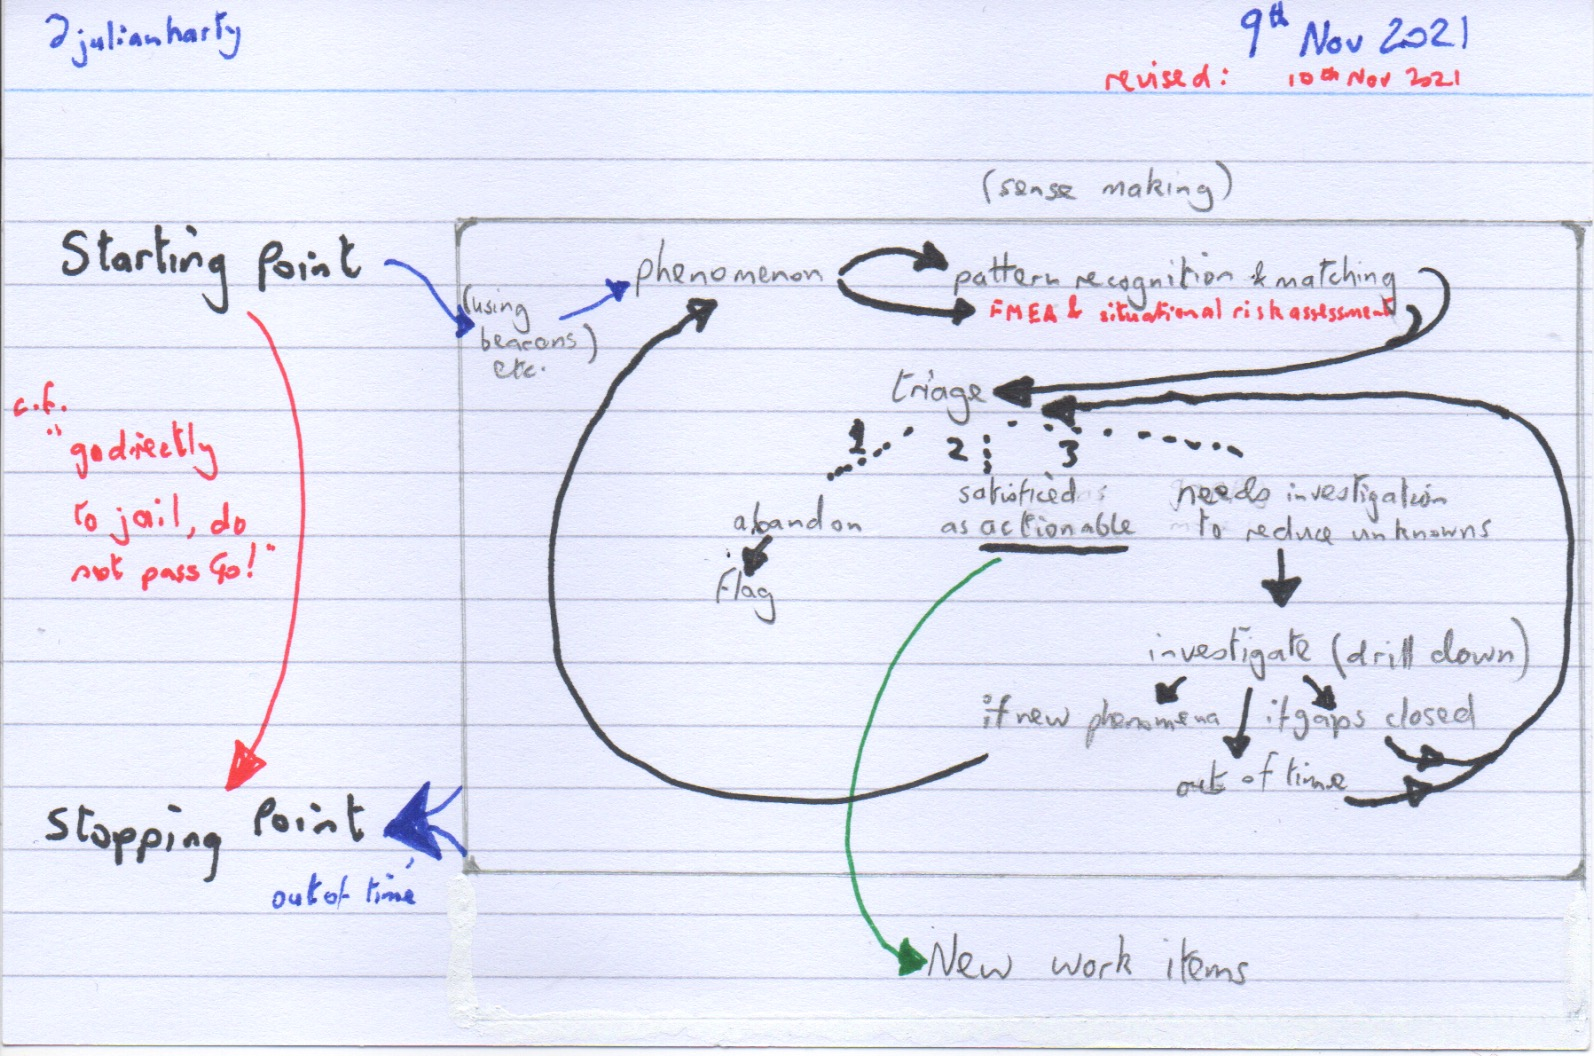
\includegraphics[width=15cm]{images/rough-sketches/practical-sense-making-process-10-nov-2021.jpeg}
    \caption{Sense-making process when development teams apply mobile analytics}
    \label{fig:practical-sense-making-process-when-dev-teams-apply-mobile-analytics}
\end{figure}


Figure~\ref{fig:practical-sense-making-process-when-dev-teams-apply-mobile-analytics} illustrates the sense-making and triage process used by development teams which shares various similarities with sense-making from a research perspective. These similarities mean the researcher and the practitioner may also share similar practices in terms of their analysis of phenomena found in mobile analytics tools. The triage and drill-down may be repeated several times where there is sufficient potential value in performing further investigation. 

The impact of reported failures is combined with situational-risk-assessment as a part of the decision-making process performed by developers during triage; for instance to consider whether this reported issue is worth addressing in the current development cycle, (\textit{e.g.} in the current sprint for teams who use sprints for work planning. Developers have to consider multiple criteria including personal, project, and product implications of making code and/or operational changes. An untested hypothesis for their approach is introduced in the discussion chapter on page \pageref{discussion-decision-making-by-dev-teams-section}.

\newthought{Premature satisfaction}

Many of the developers were often satisficed with what the mobile analytics tools reported - where they accepted local optima (determined through a combination of observation and asking the app devs), \textit{e.g.} they accepted the `top' crash cluster as the worst one. Therefore, if there are flaws in what is being reported the effects of those flaws may permeate into the results of what the developers \textit{do} and \textit{don't} do. 

\newthought{Triaging failures}

The GTAF team used a heuristic when deciding which crashes to fix. They chose to work on those perceived as relatively easy to fix and which affected many users. They provided examples of easier to fix exceptions: NullPointerException~\footnote{Helpfully discussed in \href{https://en.wikibooks.org/wiki/Java\_Programming/Preventing\_NullPointerException}{en.wikibooks.org/wiki/Java\_Programming/Preventing\_NullPointerException}.} and IndexOutOfBoundsException~\footnote{Discussed in \url{https://stackoverflow.com/a/40006381/340175}} versus some they found harder to fix: IllegalStateException~\footnote{An example of an Android specific crash is discussed in~\url{https://stackoverflow.com/questions/55158930/illegalstateexception-caused-by-intent}} and native crashes~\footnote{Useful Android documentation on diagnosing native crashes \url{https://source.android.com/devices/tech/debug/native-crash}}.


\section{What's ``good enough"? and for whom?}

\section{Using issue databases}
The GTAF team create issues in their online issue database \url{https://gitlab.com/greentech/} for crashes and include links to the source information in the respective mobile analytics tool. These links are a) only available to people who already have access to the mobile analytics account, and b) are ephemeral.

